
% This LaTeX was auto-generated from an M-file by MATLAB.
% To make changes, update the M-file and republish this document.

\documentclass{article}
\usepackage{graphicx}
\usepackage{color}
\usepackage{listings}
\usepackage[framed]{mcode}
\usepackage{fullpage}
\usepackage{amsmath}
\usepackage[utf8x]{inputenc}
\usepackage{import}
\usepackage{setspace}
\usepackage{hyperref}
\definecolor{lightgray}{gray}{0.5}
\setlength{\parindent}{0pt}

\begin{document}

    
    
%\section*{}


\title{BE 521: Homework 1 \\{\normalsize Exploring Neural Signals} \\{\normalsize Spring 2021}}
\author{33 points}
\date{Due: Tuesday 2/2/2021 10 PM}
\maketitle
\textbf{Objective:} Working with the IEEG Portal to explore different Neural signals


\begin{center}
\author{Saif Khawaja \\
  \normalsize Collaborators: Raveen K\\}
\end{center}


\section{Seizure Activity (16 pts)}
The dataset \texttt{I521\_A0001\_D002} contains an example of human intracranial EEG (iEEG) data displaying seizure activity. It is recorded from a single channel (2 electrode contacts) implanted in the hippocampus of a patient with temporal lobe epilepsy being evaluated for surgery. In these patients, brain tissue where seizures are seen is often resected. You will do multiple comparisons with this iEEG data and the unit activity that you worked with in Homework 0 \texttt{(I521\_A0001\_D001)}. You will have to refer to that homework and/or dataset for these questions.
\begin{enumerate}
 \item Retrieve the dataset in MATLAB using the IEEGToolbox and generate a \emph{session} variable as before (No need to report the output this time). What is the sampling rate of this data? What is the maximum frequency of the signal content that we can resolve? (2 pts)

\begin{lstlisting}
% The sampling rate is 200 Hz. We can resolve a maximum frequency of 200 Hz
% / 2 = 100 Hz.

session = IEEGSession('I521_A0001_D002', 'saifkhawaja', 'sai_ieeglogin.bin')

session.data

Hz = session.data.sampleRate
\end{lstlisting}

\color{lightgray} \begin{lstlisting}IEEGSETUP: Adding 'ieeg-matlab.jar' to dynamic classpath
Warning: Objects of edu/upenn/cis/db/mefview/services/TimeSeriesDetails class
exist - not clearing java 
Warning: Objects of edu/upenn/cis/db/mefview/services/TimeSeriesInterface class
exist - not clearing java 
IEEGSETUP: Found log4j on Java classpath.
URL: https://www.ieeg.org/services
Client user: saifkhawaja
Client password: ****

session = 

  <a href="matlab:help('IEEGSession')">IEEGSession</a>:

      server: 'ieeg.org'
    userName: 'saifkhawaja'
        data: [1x1 IEEGDataset]

  <a href="matlab:methods(IEEGSession)">Methods</a>, <a href="matlab:IEEGObject.openPortalSite()">main.ieeg.org</a>


ans = 

  <a href="matlab:help('IEEGDataset')">IEEGDataset</a>:

         snapName: 'I521_A0001_D002'
          montage: As Recorded
           filter: 'No Filter'
         resample: 'Not resampled'
       sampleRate: 200
           values: 
    channelLabels: [1x2 cell]
         annLayer: []
      rawChannels: [1x1 IEEGTimeseries]
      allMontages: [1x44 IEEGMontage]

  <a href="matlab:methods(IEEGDataset)">Methods</a>, <a href="matlab:IEEGObject.openPortalSite()">main.ieeg.org</a>


Hz =

   200

\end{lstlisting} \color{black}

 \item How does the duration of this recording compare with the recording from HW0 \texttt{(I521\_A0001\_D001)}? (2 pts)

\begin{lstlisting}
% Obtain the duration of the recording for channel 1 (retuyrned in microseconds).

durationInSec = session.data(1).rawChannels(1).get_tsdetails.getDuration / 1e6

% durationInSec = 644.9950 seconds, which contrasts with 10s recorded in HW0.
\end{lstlisting}

\color{lightgray} \begin{lstlisting}
durationInSec =

  644.9950

\end{lstlisting} \color{black}

 \item Using the time-series visualization functionality of the IEEG Portal, provide a screenshot of the first 500 ms of data from this recording. (2 pts)

\begin{lstlisting}
% 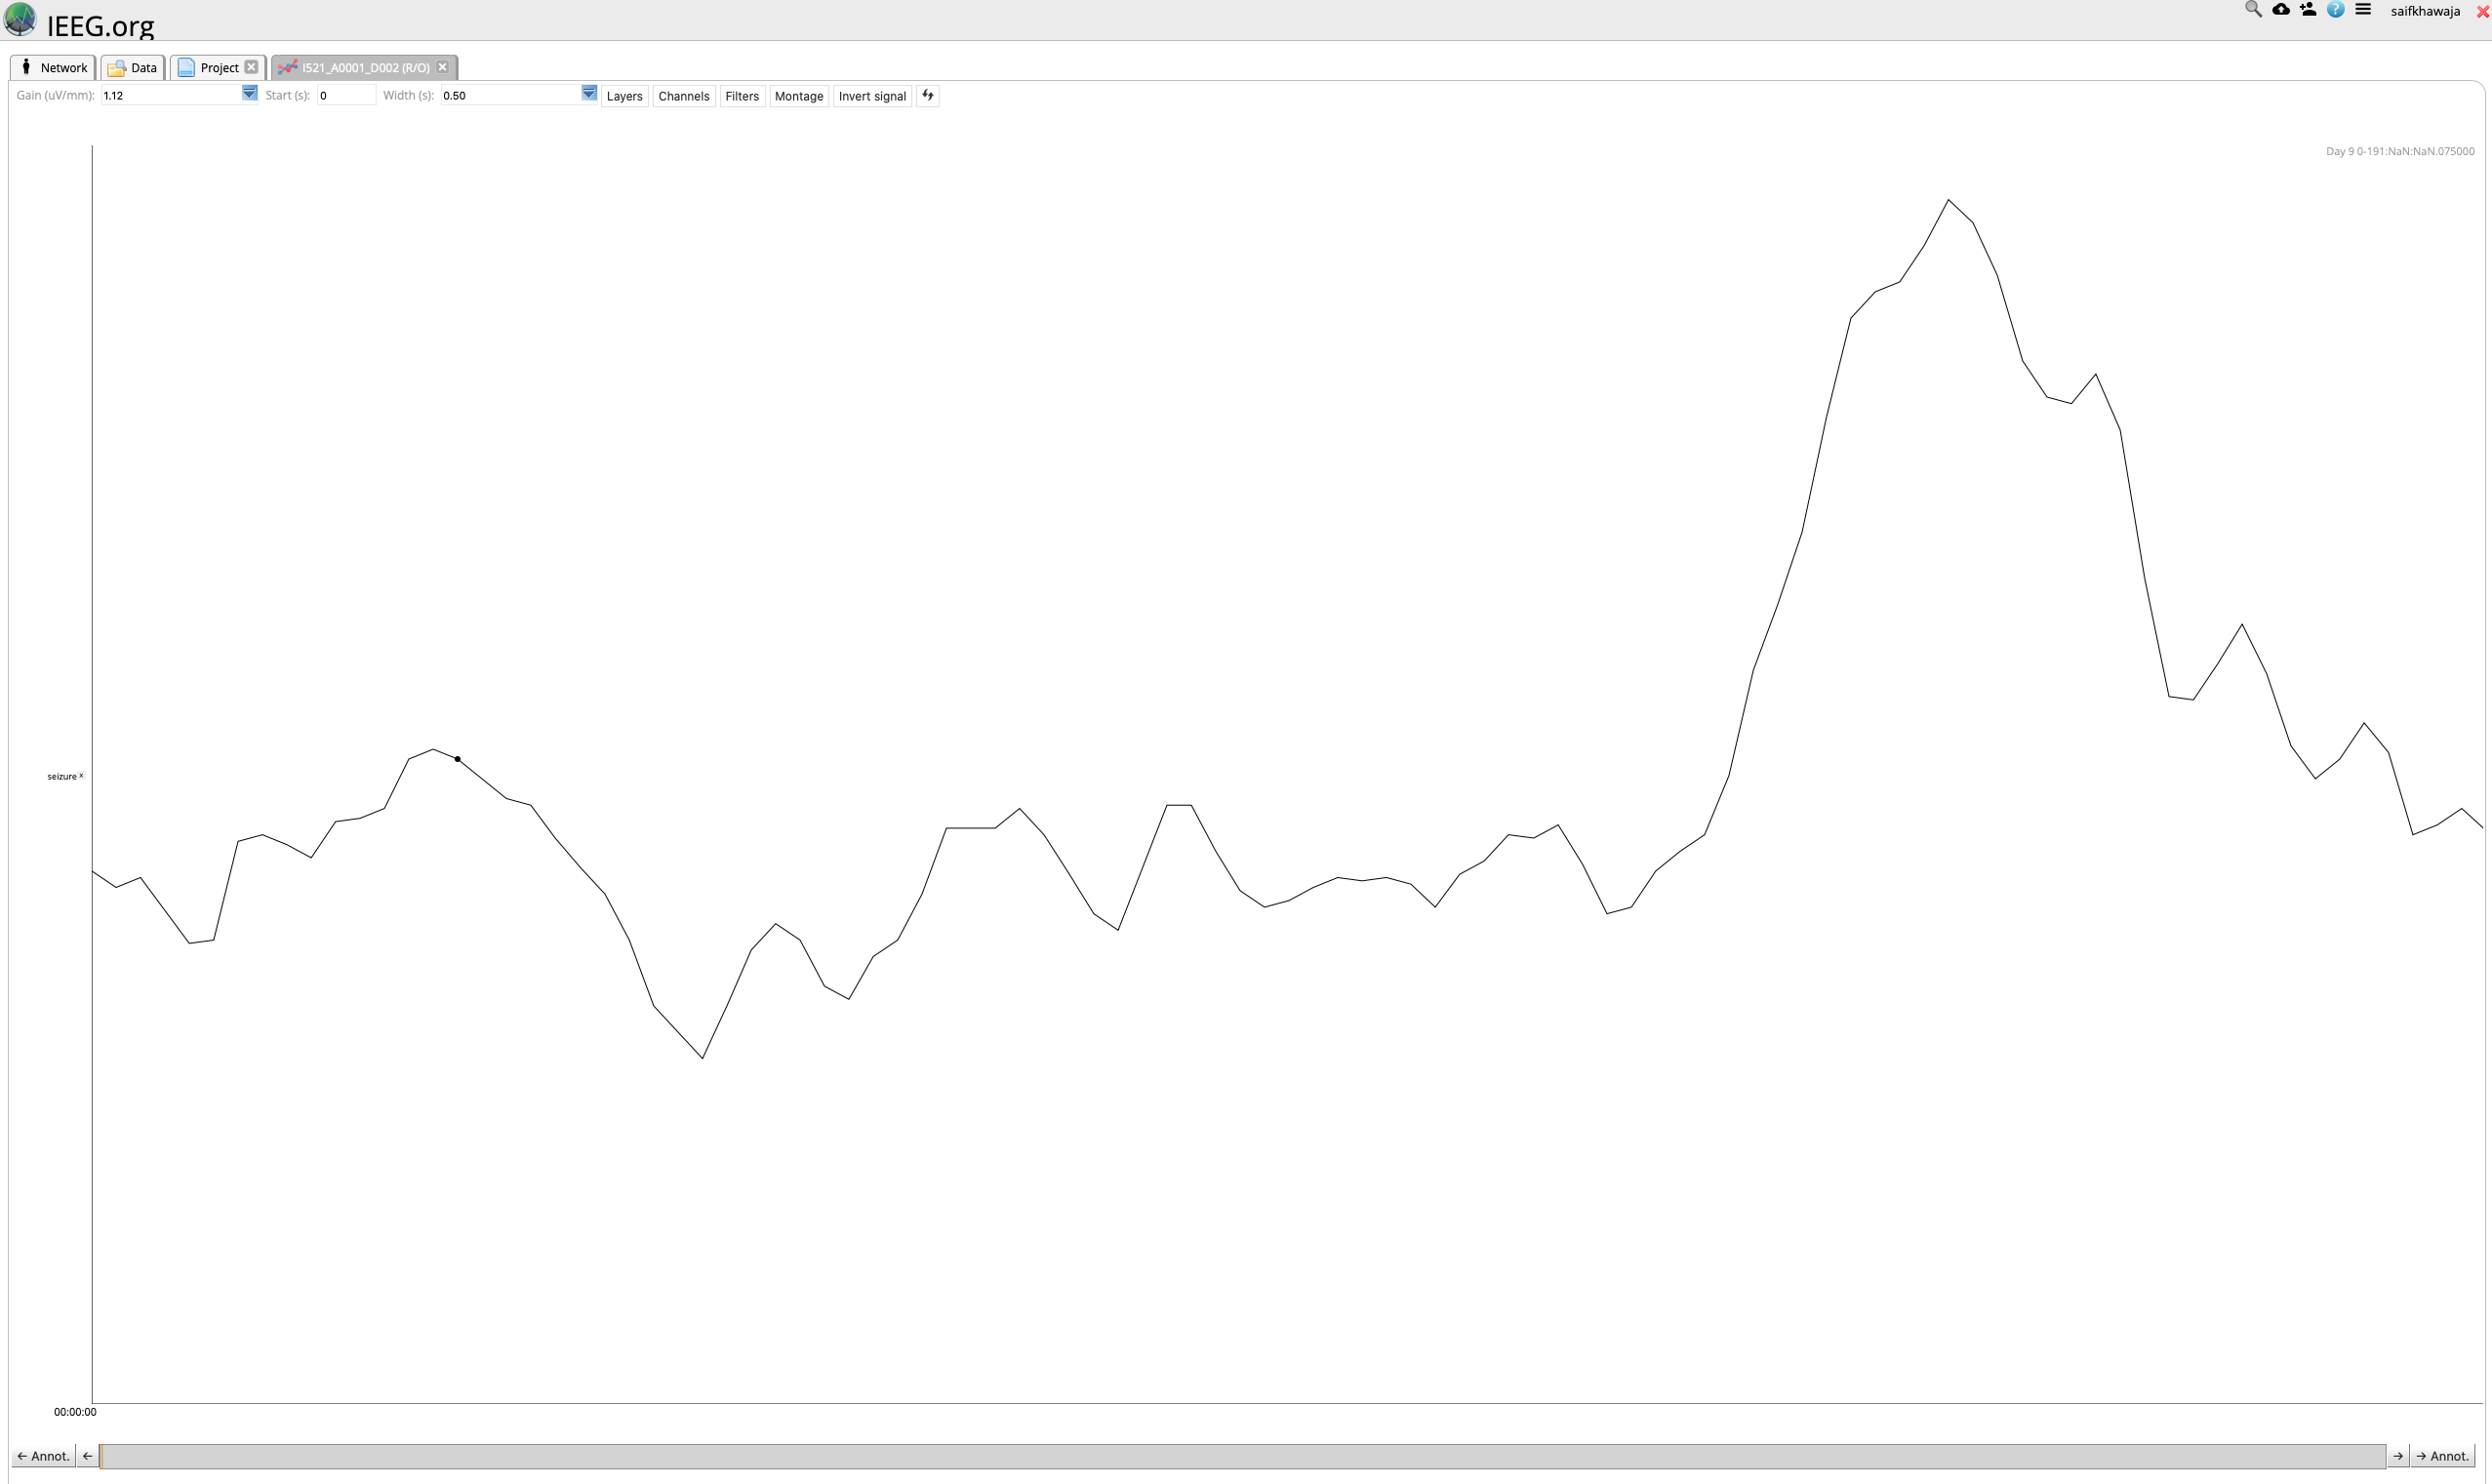
\includegraphics[scale=0.3]{/Users/saif/Documents/GitHub/braincomputerinterfaces/Homeworks/HW1/signal.png}\\
\end{lstlisting}

 \item Compare the activity in this sample with the data from HW0.  What differences do you notice in the amplitude and frequency characteristics? (2 pts)

\begin{lstlisting}
% Re-obtain HW1 data initially:

session = IEEGSession('I521_A0001_D002', 'saifkhawaja', 'sai_ieeglogin.bin');

session.data;

durationInSec = session.data(1).rawChannels(1).get_tsdetails.getDuration / 1e6;

nr = ceil((session.data.rawChannels(1).get_tsdetails.getEndTime)/1e6*(session.data.sampleRate));
allData = session.data.getvalues(1:nr,1);

sr2 = 200;

ms1 = allData(1:0.5*sr2);
peak1 = max(ms1)

% Initialize session and pull HW0 data:

session0 = IEEGSession('I521_A0001_D001', 'saifkhawaja', 'sai_ieeglogin.bin');

session0.data;

sr1 = 32051;
nr = ceil((session0.data.rawChannels(1).get_tsdetails.getEndTime)/1e6*session0.data.sampleRate);
allData = session0.data.getvalues(1:nr, 1);

ms0 = allData(1:0.5*sr1);
peak0 = max(ms0)

% As we can see here, the peak amplitude of HW0 is much larger.

A_D001 = mean(ms0)
A_D002 = mean(ms1)

% As we can see here, the average amplitude of HW0 is much smaller so has
% less variation in signal over the period of data collected.
% Additionally, the frequency of 001 is much higher.
\end{lstlisting}

\color{lightgray} \begin{lstlisting}IEEGSETUP: Adding 'ieeg-matlab.jar' to dynamic classpath
Warning: Objects of edu/upenn/cis/db/mefview/services/TimeSeriesDetails class
exist - not clearing java 
Warning: Objects of edu/upenn/cis/db/mefview/services/TimeSeriesInterface class
exist - not clearing java 
IEEGSETUP: Found log4j on Java classpath.
URL: https://www.ieeg.org/services
Client user: saifkhawaja
Client password: ****

peak1 =

   167

IEEGSETUP: Adding 'ieeg-matlab.jar' to dynamic classpath
Warning: Objects of edu/upenn/cis/db/mefview/services/TimeSeriesDetails class
exist - not clearing java 
Warning: Objects of edu/upenn/cis/db/mefview/services/TimeSeriesInterface class
exist - not clearing java 
IEEGSETUP: Found log4j on Java classpath.
URL: https://www.ieeg.org/services
Client user: saifkhawaja
Client password: ****
Warning: Integer operands are required for colon operator when used as index. 

peak0 =

  131.8830


A_D001 =

    0.0041


A_D002 =

   -7.7000

\end{lstlisting} \color{black}

 \item The unit activity sample in \texttt{(I521\_A0001\_D001)} was high-pass filtered to remove low-frequency content. Assume that the seizure activity in \texttt{(I521\_A0001\_D002)} has not been high-pass filtered. Given that the power of a frequency band scales roughly as $1/f$, how might these differences in preprocessing contribute to the differences you noted in the previous question? (There is no need to get into specific calculations here. We just want general ideas.) (3 pts)

\begin{lstlisting}
% <latex>
%  \item The removal of noise through the high-pass filtering in
%  pre-processing cleaning of the data results in more prominent striations
%  in the data. There are more oscillations in D001 than in D002, which
%  would likely be resolved if the same pre-processing was implemented in D002.
% Similarly, if we had preprovessed D002, we would observe flatter
% oscillations and lower amplitudes because, as reference in the 1/f in
% question, the power scales exponentially as frequency shrinks as the
% amplitude increases. This means that the waves on the reading have lower
% power and would flatten out if removed. Compared to D001, this would be
% flatter and if we did not remove the lower frequencies in D001 we would
% observe larger amplitude and sharper disparations in spikes as the signal
% would have a larger amount of content in lower frequencies. Since D002
% has not been high pass filtered, we see a much larger amplitude variation
% during onsets responsible.
% </latex>
\end{lstlisting}

 \item Two common methods of human iEEG are known as electrocorticography (ECoG) and stereoelectroencephalography (SEEG). For either of these paradigms (please indicate which you choose), find and report at least two of the following electrode characteristics: shape, material, size. Please note that exact numbers aren't required, and please cite any sources used. (3 pts)

\begin{lstlisting}
% Electrocorticography (ECoG) places electrodes directly on exposed
% surfaces of the brain to record cerebral cortex activity. ECoG electrode
% arrays are typically organized as sixteen strile stainless steel carbon
% tipped electrodes made of platinum, platinum-indium alloys or gold. Grid
% electrodesa are widely used and have between 4 and 256 contacts.
% Spacing is normally 1cm and individual electrodes are ~5mm in diameter.
%
% References:
% Mesgarani, N; Chang, EF (2012). "Selective cortical representation of
% attended speaker in multi-talker speech perception". Nature. 485 (7397):
% 233–6. Bibcode:2012Natur.485..233M. doi:10.1038/nature11020.
% Schuh, L; Drury, I (1996). "Intraoperative electrocorticography and
% direct cortical electrical stimulation". Seminars in Anesthesia. 16:
% 46–55. doi:10.1016/s0277-0326(97)80007-4
\end{lstlisting}

 \item What is a local field potential? How might the  characteristics of human iEEG electrodes cause them to record local field potentials as opposed to multiunit activity, which was the signal featured in HW0 as recorded from 40 micron Pt-Ir microwire electrodes? (2 pts)

\begin{lstlisting}
% A local field potential is an extracellular signal generated from ion
% concentration imbalances outside of cells. The potentials are generated
% by the voltage from charge separation across this ion concentration
% difference (relative excitatory and inhibitory dendric potentials). In
% contrast, multiunit activity takes the mean of spikes in close proximity
% to an individual electrode.
%
% iEEG electrodes can record local field potentials because of their
% comparitively large size (40 micron vs. 5mm diameter) to MUA electrodes.
% This means the signals recorded and read are a summation of multiple
% neuron potentials. The 40 micron Pt-Ir electrodes pick up signals from
% multiunit activity because of their size and the much higher sampling
% rate required for recording the minutia in adjustments.

% Reference:
% Stacey WC, Kellis S, Greger B, et al. Potential for unreliable
% interpretation of EEG recorded with microelectrodes. Epilepsia.
% 2013;54(8):1391-1401. doi:10.1111/epi.12202
\end{lstlisting}

\end{enumerate}


\section{Evoked Potentials (17 pts)}
The data in \texttt{I521\_A0001\_D003} contains an example of a very common type of experiment and neuronal signal, the evoked potential (EP). The data show the response of the whisker barrel cortex region of rat brain to an air puff stimulation of the whiskers. The \texttt{stim} channel shows the stimulation pattern, where the falling edge of the stimulus indicates the start of the air puff, and the rising edge indicates the end. The \texttt{ep} channel shows the corresponding evoked potential.
Once again, play around with the data on the IEEG Portal, in particular paying attention to the effects of stimulation on EPs. You should observe the data with window widths of 60 secs as well as 1 sec. Again, be sure to explore the signal gain to get a more accurate picture. Finally, get a sense for how long the trials are (a constant duration) and how long the entire set of stimuli and responses are.


\begin{enumerate}
 \item Based on your observations, should we use all of the data or omit some of it? (There's no right answer, here, just make your case either way in a few sentences.) (2 pts)

\begin{lstlisting}
% While there is a large similarity in most of the readings that there is a
% noticeable peak, many of the recorded signals also have a large trough
% (and sometimes multiple troughs). Moreover, some trials had multiple peaks.
% These indicate there could be additional stimuli (lights, noises, and
% other sensory inputs) that triggered a response in the rat, and therefore
% these recordings should be removed as they do not isolate the signal we are
% looking for.
\end{lstlisting}

 \item Retrieve the \texttt{ep} and \texttt{stim} channel data in MATLAB. What is the average latency (in ms) of the peak response to the stimulus onset over all trials? (Assume stimuli occurs at exactly 1 second intervals)(3 pts)

\begin{lstlisting}
% Initialize session for dataset 003 and pull information

session3 = IEEGSession('I521_A0001_D003', 'saifkhawaja', 'sai_ieeglogin.bin');

session3.data(1)

sr = session3.data.sampleRate;

nr = ceil((session3.data.rawChannels(1).get_tsdetails.getEndTime)/1e6*sr);
data3 = session3.data.getvalues(1:nr, 1:2);

ep = data3(:,1);
stim = data3(:,2);

% Obtain durtation and sample rate to use in calculation for peak difs

durationInUSec = session3.data(1).rawChannels(1).get_tsdetails.getDuration;
durationInSec = durationInUSec / 1e6;

% Calculate peak locations and store them in peakpoints array

times=(0:1:durationInSec);


mult = length(times);

initial = 1;
final = sr;

peakpoints = [];

for i = 1:mult
    mult=ep(initial:final);

    [peak, index] = max(mult);
    index = index/sr;
    peakpoints(i) = index;

    initial = final + 1;
    final = final + sr;
end

average_latency = mean(peakpoints)

% The mean of the latency time is 0.162 seconds as calculated above.
\end{lstlisting}

\color{lightgray} \begin{lstlisting}IEEGSETUP: Adding 'ieeg-matlab.jar' to dynamic classpath
Warning: Objects of edu/upenn/cis/db/mefview/services/TimeSeriesDetails class
exist - not clearing java 
Warning: Objects of edu/upenn/cis/db/mefview/services/TimeSeriesInterface class
exist - not clearing java 
IEEGSETUP: Found log4j on Java classpath.
URL: https://www.ieeg.org/services
Client user: saifkhawaja
Client password: ****

ans = 

  <a href="matlab:help('IEEGDataset')">IEEGDataset</a>:

         snapName: 'I521_A0001_D003'
          montage: As Recorded
           filter: 'No Filter'
         resample: 'Not resampled'
       sampleRate: 2713
           values: 
    channelLabels: [2x2 cell]
         annLayer: []
      rawChannels: [1x2 IEEGTimeseries]
      allMontages: [1x44 IEEGMontage]

  <a href="matlab:methods(IEEGDataset)">Methods</a>, <a href="matlab:IEEGObject.openPortalSite()">main.ieeg.org</a>


average_latency =

    0.1622

\end{lstlisting} \color{black}

 \item In neuroscience, we often need to isolate a small neural signal buried under an appreciable amount of noise.  One technique to accomplish this is called the spike triggered average, sometimes called signal averaging. This technique assumes that the neural response to a repetitive stimulus is constant (or nearly so), while the noise fluctuates from trial to trial - therefore averaging the evoked response over many trials will isolate the signal and average out the noise.
 Construct a spike triggered average plot for the data in \texttt{I521\_A0001\_D003}.  Plot the average EP in red.  Using the commands \texttt{hold on} and \texttt{hold off} as well as \texttt{errorbar} and \texttt{plot}, overlay error bars at each time point on the plot to indicate the standard deviation of the responses at any given time point.  Plot the standard deviation error bars in gray (RGB value: [0.7 0.7 0.7]). Make sure to give a proper legend along with your labels. (4 pts)

\begin{lstlisting}
% Set up

session3 = IEEGSession('I521_A0001_D003', 'saifkhawaja', 'sai_ieeglogin.bin');

session3.data(1)

nr = ceil((session3.data.rawChannels(1).get_tsdetails.getEndTime)/1e6*session3.data.sampleRate);
data3 = session3.data.getvalues(1:nr, 1:2);

ep = data3(:, 1);
stim = data3(:, 2);

% Obtain duration and sample rate

durationInSec = (session3.data(1).rawChannels(1).get_tsdetails.getDuration) / 1e6;
sr = session3.data.sampleRate;

% Prepare for STAP

times = ceil(0:1:durationInSec);

average_m = [];

% Parse readings and store

initial = 1;
final = sr;

for i = 1:length(times)
    window = ep(initial:final);
    average_m(i,:) = window;

    initial = final + 1;
    final = final + sr;
end

figure('Color','white')
errorbar(0:1/sr:1-(1/sr), mean(average_m, 1), std(average_m, 1), 'Color', [0.7 0.7 0.7])

hold on
plot(0:1/sr:1-(1/sr), mean(average_m, 1))
xlabel('Time (s)')
ylabel('Amplitude (uV)')
legend('Error via Standard Deviation', 'Average Evoked Potential')
title('Spike Triggered Average')
hold off
\end{lstlisting}

\color{lightgray} \begin{lstlisting}IEEGSETUP: Adding 'ieeg-matlab.jar' to dynamic classpath
Warning: Objects of edu/upenn/cis/db/mefview/services/TimeSeriesDetails class
exist - not clearing java 
Warning: Objects of edu/upenn/cis/db/mefview/services/TimeSeriesInterface class
exist - not clearing java 
IEEGSETUP: Found log4j on Java classpath.
URL: https://www.ieeg.org/services
Client user: saifkhawaja
Client password: ****

ans = 

  <a href="matlab:help('IEEGDataset')">IEEGDataset</a>:

         snapName: 'I521_A0001_D003'
          montage: As Recorded
           filter: 'No Filter'
         resample: 'Not resampled'
       sampleRate: 2713
           values: 
    channelLabels: [2x2 cell]
         annLayer: []
      rawChannels: [1x2 IEEGTimeseries]
      allMontages: [1x44 IEEGMontage]

  <a href="matlab:methods(IEEGDataset)">Methods</a>, <a href="matlab:IEEGObject.openPortalSite()">main.ieeg.org</a>

\end{lstlisting} \color{black}

 \item
  \begin{enumerate}
	\item We often want to get a sense for the amplitude of the noise in a single trial. Propose a method to do this (there are a few reasonably simple methods, so no need to get too complicated). Note: do not assume that the signal averaged EP is the ``true'' signal and just subtract it from that of each trial, because whatever method you propose should be able to work on the signal from a single trial or from the average of the trials. (4 pts)

\begin{lstlisting}
% We can identify and reduce noise through a number of methods, one of
% which is taking a moving average across short time bursts. A moving
% average is a succession of averages derived from successive segments
% (typically of constant size and overlapping) of a series of values.
% In this context, we can average the successive amplitudes of n amount of
% neighbouring points (say 30) using the movmean function. After
% subtracting the generated signal from the original, we can average the
% noise out to approximate noise presence over time, which can the be
% averaged again for mean noise presence. This does operate on the premise
% that the noise is equidistant from the calculated initial mean (a little
% trivial but it gets the job done).
\end{lstlisting}

	\item Show with a few of the EPs (plots and/or otherwise) that your method gives reasonable results. (1 pt)

\begin{lstlisting}
% First four trials below. All values except x are redeclared per trial as each new cycle requires redeclaration. Looking at the figures, this seems reasonable as a method.

noise_init_1 = 1;
noise_final_1 = sr;
window_pass = ep(noise_init_1:noise_final_1);
mvng_avg = movmean(window_pass, 30);

x_vals = 0:1/sr:1-(1/sr);

figure
subplot(4, 1, 1, 'align')
plot(x_vals, mvng_avg, 'Linewidth', 3, 'Color', 'b')
xlabel('T (s)')
ylabel('A (uV)')
title('Pre-Processed Noise Reduced EP 1')
hold on
plot(x_vals, window_pass, 'Color','y')
legend('Adjusted Signal','Unadjusted Signal')
hold off

noise_init_2 = noise_final_1 + 1;
noise_final_2 =noise_final_1 + sr;

window_pass = ep(noise_init_2:noise_final_2);
mvng_avg = movmean(window_pass, 30);

subplot(4, 1, 2, 'align')
plot(x_vals, mvng_avg, 'Linewidth', 3, 'Color','b')
xlabel('T (s)')
ylabel('A (uV)')
title('Pre-Processed Noise Reduced EP 2')
hold on
plot(x_vals, window_pass, 'Color','y')
legend('Adjusted Signal','Unadjusted Signal')
hold off

noise_init_3 = noise_final_2 + 1;
noise_final_3 =noise_final_2 + sr;

window_pass = ep(noise_init_3:noise_final_3);
mvng_avg = movmean(window_pass, 30);

subplot(4, 1, 3, 'align')
plot(x_vals, mvng_avg, 'Linewidth', 3, 'Color','b')
xlabel('T (s)')
ylabel('A (uV)')
title('Pre-Processed Noise Reduced EP 3')
hold on
plot(x_vals, window_pass, 'Color','y')
legend('Adjusted Signal','Unadjusted Signal')
hold off

noise_init_4 = noise_final_3 + 1;
noise_final_4 =noise_final_3 + sr;

window_pass = ep(noise_init_4:noise_final_4);
mvng_avg = movmean(window_pass, 30);

subplot(4, 1, 4, 'align')
plot(x_vals, mvng_avg, 'Linewidth', 3, 'Color','b')
xlabel('T (s)')
ylabel('A (uV)')
title('Pre-Processed Noise Reduced EP 4')
hold on
plot(x_vals, window_pass, 'Color','y')
legend('Adjusted Signal','Unadjusted Signal')
hold off
\end{lstlisting}

	\item
    \begin{enumerate}
        \item Apply your method on each individual trial and report the mean noise amplitude across all trials. (1 pt)

\begin{lstlisting}
initial = 1;
final = sr;

for i=1:length(times)
    delta = mean(abs(movmean(ep(initial:final), 30) - ep(initial:final)));
    noise(i) = delta;

    initial = final + 1;
    final = final + sr;
end

mean(noise)

% As shown above, the mean noise is 384.94 uV.
\end{lstlisting}

\color{lightgray} \begin{lstlisting}
ans =

  384.9384

\end{lstlisting} \color{black}

        \item Apply your method on the signal averaged EP and report its noise. (1 pt)

\begin{lstlisting}
mean(mean(abs(mean(average_m, 1) - movmean(mean(average_m, 1), 30))))

% As shown above, signal averaged noise is 44.93 uV.
\end{lstlisting}

\color{lightgray} \begin{lstlisting}
ans =

   44.9340

\end{lstlisting} \color{black}

	    \item Do these two values make sense? Explain. (1 pt)

\begin{lstlisting}
% Yes — noise in the averaged EP signal had already been partially
% removed when we took the mean. If we look at the values, the signal
% averaged EP has a 44.93 uV noise content, which is comparitively small to
% the 384.94 uV of mean amplitude of noise across all the trials.  This is
% an order of magnitude difference, which indicates that the signal is more
% prominent than the noise as we hope.
\end{lstlisting}

    \end{enumerate}
  \end{enumerate}
\end{enumerate}




\end{document}
    
